\documentclass[11pt,utf8,notheorems,compress,t]{beamer}
\usepackage{etex}

\usepackage{pgfpages}
\usepackage[export]{adjustbox}

% Workaround for the issue described at
% https://tex.stackexchange.com/questions/164406/beamer-using-href-in-notes.
\newcommand{\fixedhref}[2]{\makebox[0pt][l]{\hspace*{\paperwidth}\href{#1}{#2}}\href{#1}{#2}}

\usepackage[english]{babel}

\usepackage{graphbox}
\usepackage{mathtools}
\usepackage{booktabs}
\usepackage{stmaryrd,wasysym}
\usepackage{bussproofs}
\usepackage{xspace}
\usepackage{amssymb}
\usepackage{array}
\usepackage{ragged2e}
\usepackage{multicol}
\usepackage{tabto}
\usepackage{xstring}
\usepackage{ifthen}
\usepackage[normalem]{ulem}
\usepackage[all]{xy}
\xyoption{rotate}
\usepackage{tikz}
\usetikzlibrary{calc,shapes,shapes.callouts,shapes.arrows,patterns,fit,backgrounds,decorations.pathmorphing,positioning}
\hypersetup{colorlinks=true}

\newcommand*\circled[1]{\tikz[baseline=(char.base)]{%
  \node[shape=circle,draw,inner sep=1pt] (char) {#1};}}

\DeclareFontFamily{U}{bbm}{}
\DeclareFontShape{U}{bbm}{m}{n}
   {  <5> <6> <7> <8> <9> <10> <12> gen * bbm
      <10.95> bbm10%
      <14.4>  bbm12%
      <17.28><20.74><24.88> bbm17}{}
\DeclareFontShape{U}{bbm}{m}{sl}
   {  <5> <6> <7> bbmsl8%
      <8> <9> <10> <12> gen * bbmsl
      <10.95> bbmsl10%
      <14.4> <17.28> <20.74> <24.88> bbmsl12}{}
\DeclareFontShape{U}{bbm}{bx}{n}
   {  <5> <6> <7> <8> <9> <10> <12> gen * bbmbx
      <10.95> bbmbx10%
      <14.4> <17.28> <20.74> <24.88> bbmbx12}{}
\DeclareFontShape{U}{bbm}{bx}{sl}
   {  <5> <6> <7> <8> <9> <10> <10.95> <12> <14.4> <17.28>%
      <20.74> <24.88> bbmbxsl10}{}
\DeclareFontShape{U}{bbm}{b}{n}
   {  <5> <6> <7> <8> <9> <10> <10.95> <12> <14.4> <17.28>%
      <20.74> <24.88> bbmb10}{}
\DeclareMathAlphabet{\mathbbm}{U}{bbm}{m}{n}
\SetMathAlphabet\mathbbm{bold}{U}{bbm}{bx}{n}

\usepackage{pifont}
\newcommand{\cmark}{\ding{51}}
\newcommand{\xmark}{\ding{55}}
\DeclareSymbolFont{extraup}{U}{zavm}{m}{n}
\DeclareMathSymbol{\varheart}{\mathalpha}{extraup}{86}

\graphicspath{{images/}}

\usepackage[protrusion=true,expansion=true]{microtype}

\setlength\parskip{\medskipamount}
\setlength\parindent{0pt}

\title{Revisiting divisible, injective and flabby abelian groups from a
constructive point of view}
\author{Ingo Blechschmidt}
\date{September 21th, 2022}

%\useinnertheme[shadow=true]
\setbeamerfont{block title}{size={}}

\useinnertheme{rectangles}

\usecolortheme{orchid}
\usecolortheme{seahorse}
\definecolor{mypurple}{RGB}{150,0,255}
\setbeamercolor{structure}{fg=mypurple}
\definecolor{myred}{RGB}{150,0,0}
\setbeamercolor*{title}{bg=myred,fg=white}
\setbeamercolor*{titlelike}{bg=myred,fg=white}
\setbeamercolor{frame}{bg=black}

\usefonttheme{serif}
\usepackage[T1]{fontenc}
\usepackage{libertine}

% lifted from https://arxiv.org/abs/1506.08870
\DeclareFontFamily{U}{min}{}
\DeclareFontShape{U}{min}{m}{n}{<-> udmj30}{}
\newcommand\yon{\!\text{\usefont{U}{min}{m}{n}\symbol{'210}}\!}

\newcommand{\A}{\mathcal{A}}
\newcommand{\B}{\mathcal{B}}
\newcommand{\C}{\mathcal{C}}
\newcommand{\M}{\mathcal{M}}
\renewcommand{\AA}{\mathbb{A}}
\newcommand{\BB}{\mathbb{B}}
\newcommand{\pp}{\mathbbm{p}}
\newcommand{\MM}{\mathbb{M}}
\newcommand{\E}{\mathcal{E}}
\newcommand{\F}{\mathcal{F}}
\newcommand{\FF}{\mathbb{F}}
\newcommand{\G}{\mathcal{G}}
\newcommand{\J}{\mathcal{J}}
\newcommand{\GG}{\mathbb{G}}
\renewcommand{\O}{\mathcal{O}}
\newcommand{\K}{\mathcal{K}}
\newcommand{\NN}{\mathbb{N}}
\newcommand{\QQ}{\mathbb{Q}}
\newcommand{\RR}{\mathbb{R}}
\newcommand{\TT}{\mathbb{T}}
\newcommand{\PP}{\mathbb{P}}
\newcommand{\ZZ}{\mathbb{Z}}
\newcommand{\CC}{\mathbb{C}}
\renewcommand{\P}{\mathcal{P}}
\newcommand{\aaa}{\mathfrak{a}}
\newcommand{\ppp}{\mathfrak{p}}
\newcommand{\fff}{\mathfrak{f}}
\newcommand{\defeq}{\vcentcolon=}
\newcommand{\defeqv}{\vcentcolon\equiv}
\newcommand{\Sh}{\mathrm{Sh}}
\newcommand{\GL}{\mathrm{GL}}
\newcommand{\Zar}{\mathrm{Zar}}
\newcommand{\op}{\mathrm{op}}
\newcommand{\Set}{\mathrm{Set}}
\newcommand{\Eff}{\mathrm{Ef{}f}}
\newcommand{\Sch}{\mathrm{Sch}}
\newcommand{\Aff}{\mathrm{Aff}}
\newcommand{\Ring}{\mathrm{Ring}}
\newcommand{\LocRing}{\mathrm{LocRing}}
\newcommand{\LRS}{\mathrm{LRS}}
\newcommand{\Hom}{\mathrm{Hom}}
\newcommand{\Spec}{\mathrm{Spec}}
\newcommand{\lra}{\longrightarrow}
\newcommand{\RelSpec}{\operatorname{Spec}}
\renewcommand{\_}{\mathpunct{.}\,}
\newcommand{\?}{\,{:}\,}
\newcommand{\speak}[1]{\ulcorner\text{\textnormal{#1}}\urcorner}
\newcommand{\ul}[1]{\underline{#1}}
\newcommand{\affl}{\ensuremath{{\ul{\ensuremath{\AA}}^1}}}
\newcommand{\Ll}{\text{iff}}
\newcommand{\inv}{inv.\@}
\newcommand{\seq}[1]{\mathrel{\vdash\!\!\!_{#1}}}
\newcommand{\hg}{\mathbin{:}}  % homogeneous coordinates

\setbeamertemplate{blocks}[rounded][shadow=false]

\newenvironment{indentblock}{%
  \list{}{\leftmargin\leftmargin}%
  \item\relax
}{%
  \endlist
}

% Adapted from https://latex.org/forum/viewtopic.php?t=2251 (Stefan Kottwitz)
\newenvironment<>{hilblock}{
  \begin{center}
    \begin{minipage}{9.05cm}
      \setlength{\textwidth}{9.05cm}
      \begin{actionenv}#1
        \def\insertblocktitle{}
        \par
        \usebeamertemplate{block begin}}{
        \par
        \usebeamertemplate{block end}
      \end{actionenv}
    \end{minipage}
  \end{center}}

\newenvironment{changemargin}[2]{%
  \begin{list}{}{%
    \setlength{\topsep}{0pt}%
    \setlength{\leftmargin}{#1}%
    \setlength{\rightmargin}{#2}%
    \setlength{\listparindent}{\parindent}%
    \setlength{\itemindent}{\parindent}%
    \setlength{\parsep}{\parskip}%
  }%
  \item[]}{\end{list}}

\tikzset{
  invisible/.style={opacity=0,text opacity=0},
  visible on/.style={alt={#1{}{invisible}}},
  alt/.code args={<#1>#2#3}{%
    \alt<#1>{\pgfkeysalso{#2}}{\pgfkeysalso{#3}}}
}

\newcommand{\pointthis}[3]{%
  \tikz[remember picture,baseline]{
    \node[anchor=base,inner sep=0,outer sep=0] (#2) {#2};
    \node[visible on=#1,overlay,rectangle callout,rounded corners,callout relative pointer={(0.3cm,0.5cm)},fill=blue!20] at ($(#2.north)+(-0.1cm,-1.1cm)$) {#3};
  }%
}

\tikzset{
  invisible/.style={opacity=0,text opacity=0},
  visible on/.style={alt={#1{}{invisible}}},
  alt/.code args={<#1>#2#3}{%
    \alt<#1>{\pgfkeysalso{#2}}{\pgfkeysalso{#3}}}
}

\newcommand{\hcancel}[5]{%
  \tikz[baseline=(tocancel.base)]{
    \node[inner sep=0pt,outer sep=0pt] (tocancel) {#1};
    \draw[red!80, line width=0.4mm] ($(tocancel.south west)+(#2,#3)$) -- ($(tocancel.north east)+(#4,#5)$);
  }%
}

\newcommand{\explain}[7]{%
  \tikz[remember picture,baseline]{
    \node[anchor=base,inner sep=2pt,outer sep=0,fill=#3,rounded corners] (label) {#1};
    \node[anchor=north,visible on=<#2>,overlay,rectangle callout,rounded corners,callout
    relative pointer={(0.0cm,0.5cm)+(0.0cm,#6)},fill=#3] at ($(label.south)+(0,-0.3cm)+(#4,#5)$) {#7};
  }%
}

\newcommand{\explainstub}[2]{%
  \tikz[remember picture,baseline]{
    \node[anchor=base,inner sep=2pt,outer sep=0,fill=#2,rounded corners] (label) {#1};
  }%
}

\newcommand{\squiggly}[1]{%
  \tikz[remember picture,baseline]{
    \node[anchor=base,inner sep=0,outer sep=0] (label) {#1};
    \draw[thick,color=red!80,decoration={snake,amplitude=0.5pt,segment
    length=3pt},decorate] ($(label.south west) + (0,-2pt)$) -- ($(label.south east) + (0,-2pt)$);
  }%
}

% Adapted from https://latex.org/forum/viewtopic.php?t=2251 (Stefan Kottwitz)
\newenvironment<>{varblock}[2]{\begin{varblockextra}{#1}{#2}{}}{\end{varblockextra}}
\newenvironment<>{varblockextra}[3]{
  \begin{center}
    \begin{minipage}{#1}
      \begin{actionenv}#4
        {\centering \hil{#2}\par}
	\def\insertblocktitle{}%\centering #2}
        \def\varblockextraend{#3}
	\usebeamertemplate{block begin}}{
        \par
        \usebeamertemplate{block end}
        \varblockextraend
      \end{actionenv}
    \end{minipage}
  \end{center}}

\setbeamertemplate{headline}{}

\setbeamertemplate{frametitle}{%
  \vskip0.5em%
  \leavevmode%
  \begin{beamercolorbox}[dp=1ex,center]{}%
    \begin{tikzpicture}
      \def\R{8pt}
      \node (title) {\hil{{\large\,\!\insertframetitle}}};
      \begin{pgfonlayer}{background}
        \draw[decorate, very thick, draw=mypurple!30]
          ($(title.south west) + (\R, 0)$) arc(270:180:\R) --
          ($(title.north west) + (0, -\R)$) arc(180:90:\R) --
          ($(title.north east) + (-\R, 0)$) arc(90:0:\R) --
          ($(title.south east) + (0, \R)$) arc(0:-90:\R) --
          cycle;
      \end{pgfonlayer}
    \end{tikzpicture}
  \end{beamercolorbox}%
  \vskip-0.2em%
}

\setbeamertemplate{navigation symbols}{}

\newcounter{framenumberpreappendix}
\newcommand{\backupstart}{
  \setcounter{framenumberpreappendix}{\value{framenumber}}
}
\newcommand{\backupend}{
  \addtocounter{framenumberpreappendix}{-\value{framenumber}}
  \addtocounter{framenumber}{\value{framenumberpreappendix}}
}

\newcommand{\insertframeextra}{}
\setbeamertemplate{footline}{%
  \begin{beamercolorbox}[wd=\paperwidth,ht=2.25ex,dp=1ex,right,rightskip=1mm,leftskip=1mm]{}%
    % \inserttitle
    \hfill
    \insertframenumber\insertframeextra\,/\,\inserttotalframenumber
  \end{beamercolorbox}%
  \vskip0pt%
}


\newcommand{\hil}[1]{{\usebeamercolor[fg]{item}{\textbf{#1}}}}
\newcommand{\bad}[1]{\textcolor{red!90}{\textnormal{#1}}}
\newcommand{\good}[1]{\textcolor{mypurple}{\textnormal{#1}}}

\newcommand{\bignumber}[1]{%
  \renewcommand{\insertenumlabel}{#1}\scalebox{1.2}{\!\usebeamertemplate{enumerate item}\!}
}
\newcommand{\normalnumber}[1]{%
  {\renewcommand{\insertenumlabel}{#1}\!\usebeamertemplate{enumerate item}\!}
}
\newcommand{\bigheart}{
\includegraphics{heart}}

\newcommand{\subhead}[1]{{\centering\textcolor{gray}{\hrulefill}\quad\textnormal{#1}\quad\textcolor{gray}{\hrulefill}\par}}

\newcommand{\badbox}[1]{\colorbox{red!30}{#1}}
\newcommand{\infobox}[1]{\colorbox{yellow!70}{\color{black}#1}}
\newcommand{\grayline}{\textcolor{gray}{\hspace*{-3em}\hrulefill\hspace*{-3em}}}
\newcommand{\notnot}{\emph{not~not}\xspace}

\begin{document}

\addtocounter{framenumber}{-1}

%\setbeamertemplate{headline}{\mynav{gray}{gray}{gray}}

{\usebackgroundtemplate{\begin{minipage}{\paperwidth}\vspace*{1.59cm}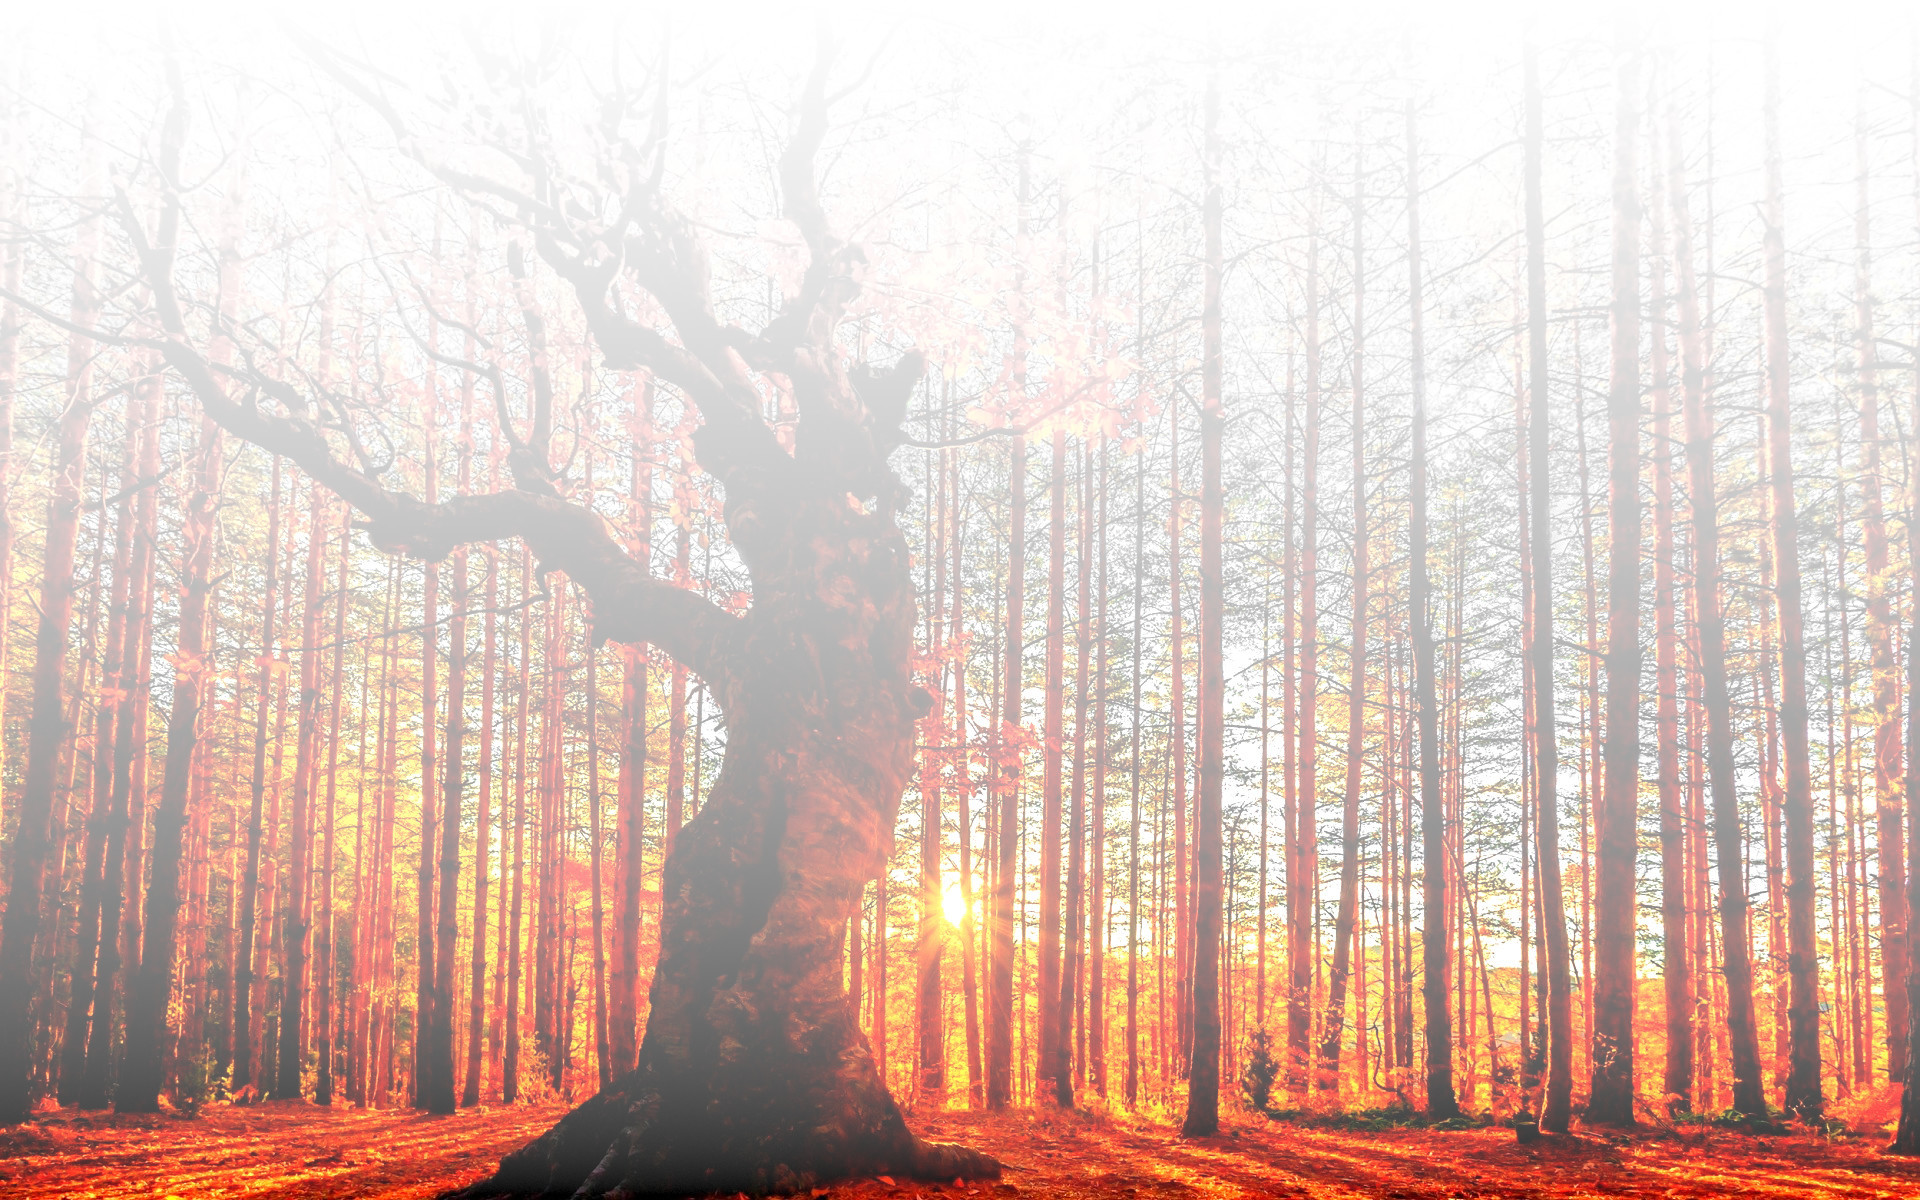
\includegraphics[width=\paperwidth]{forest-light}\end{minipage}}
\definecolor{mypurple}{RGB}{253,73,34}
\begin{frame}[c]
  \centering

  \bigskip
  \bigskip
  \bigskip
  \bigskip

  \scriptsize
  \textit{-- an invitation --}

  \setbeamercolor{block body}{bg=black!100}
  \begin{block}{}
    \centering\normalsize\color{white}
    \hil{Extraction} of \hil{programs} from \hil{proofs}
  \end{block}

  \bigskip
  \bigskip
  \bigskip
  \bigskip
  \bigskip
  \bigskip
  \bigskip

  Autumn school on \\
  \emph{Proof and Computation} \\
  in Fischbachau \\
  \ \\
  September 26th to October 1st, 2022

  Ingo Blechschmidt \\
  University of Augsburg
  \par
\end{frame}}

{\usebackgroundtemplate{\begin{minipage}{\paperwidth}\vspace*{5.95cm}
\includegraphics[width=\paperwidth]{fr1-lighter}\end{minipage}}
\begin{frame}{}
  \medskip
  \textbf{Thm.}
  For every number~$n \in \NN$, there is a prime larger than~$n$.

  {\emph{Proof.} Any prime factor of~$n! + 1$ will do.\par}
  \medskip
  \pause

  {\centering\emph{``Every constructive theorem has a computable witness.''}
  \pause
  \[
    \begin{array}{c@{\qquad}c@{\qquad}c}
      \mathrm{HA} \vdash \varphi &\Longrightarrow&
      \exists e\_ e \Vdash \varphi \\
      \text{\small constructive proof} &\longmapsto&
      \text{\small realizer}
    \end{array}
  \]}
  \pause
  \vspace*{-2.2em}

  \begin{columns}
    \begin{column}{0.45\textwidth}
      \begin{itemize}
        \item Integrated developments \\ \emph{SAT checking, \ldots}
        \item Computability theory \\ \emph{induction $\widehat{=}$ recursion, \ldots}
      \end{itemize}
    \end{column}

    \hspace*{-1em}
    \begin{column}{0.65\textwidth}
      \begin{itemize}
        \item Metatheory of constructive systems \\ \emph{provability results, \ldots}
        \item Philosophy of proof and computation \\ \emph{realizability in the real world, \ldots}
      \end{itemize}
    \end{column}
  \end{columns}

  \grayline
  \pause

  \justifying
  \textbf{Thm.} Every infinite sequence~$\alpha : \NN \to \NN$ is \emph{good}
  in that there are numbers~$i < j$ such that~$\alpha(i) \leq \alpha(j)$.

  {\emph{Proof.} By~\badbox{\textsc{lem}}, there is a minimal value~$\alpha(i)$.
  Set~$j \defeq i + 1$.\par}

  {\centering\emph{``Every theorem has a computable* witness.''} \\ \scriptsize
  * with monadic side effects\par}
\end{frame}}

% 
\includegraphics[width=3cm]{lovelace-babbage}
% 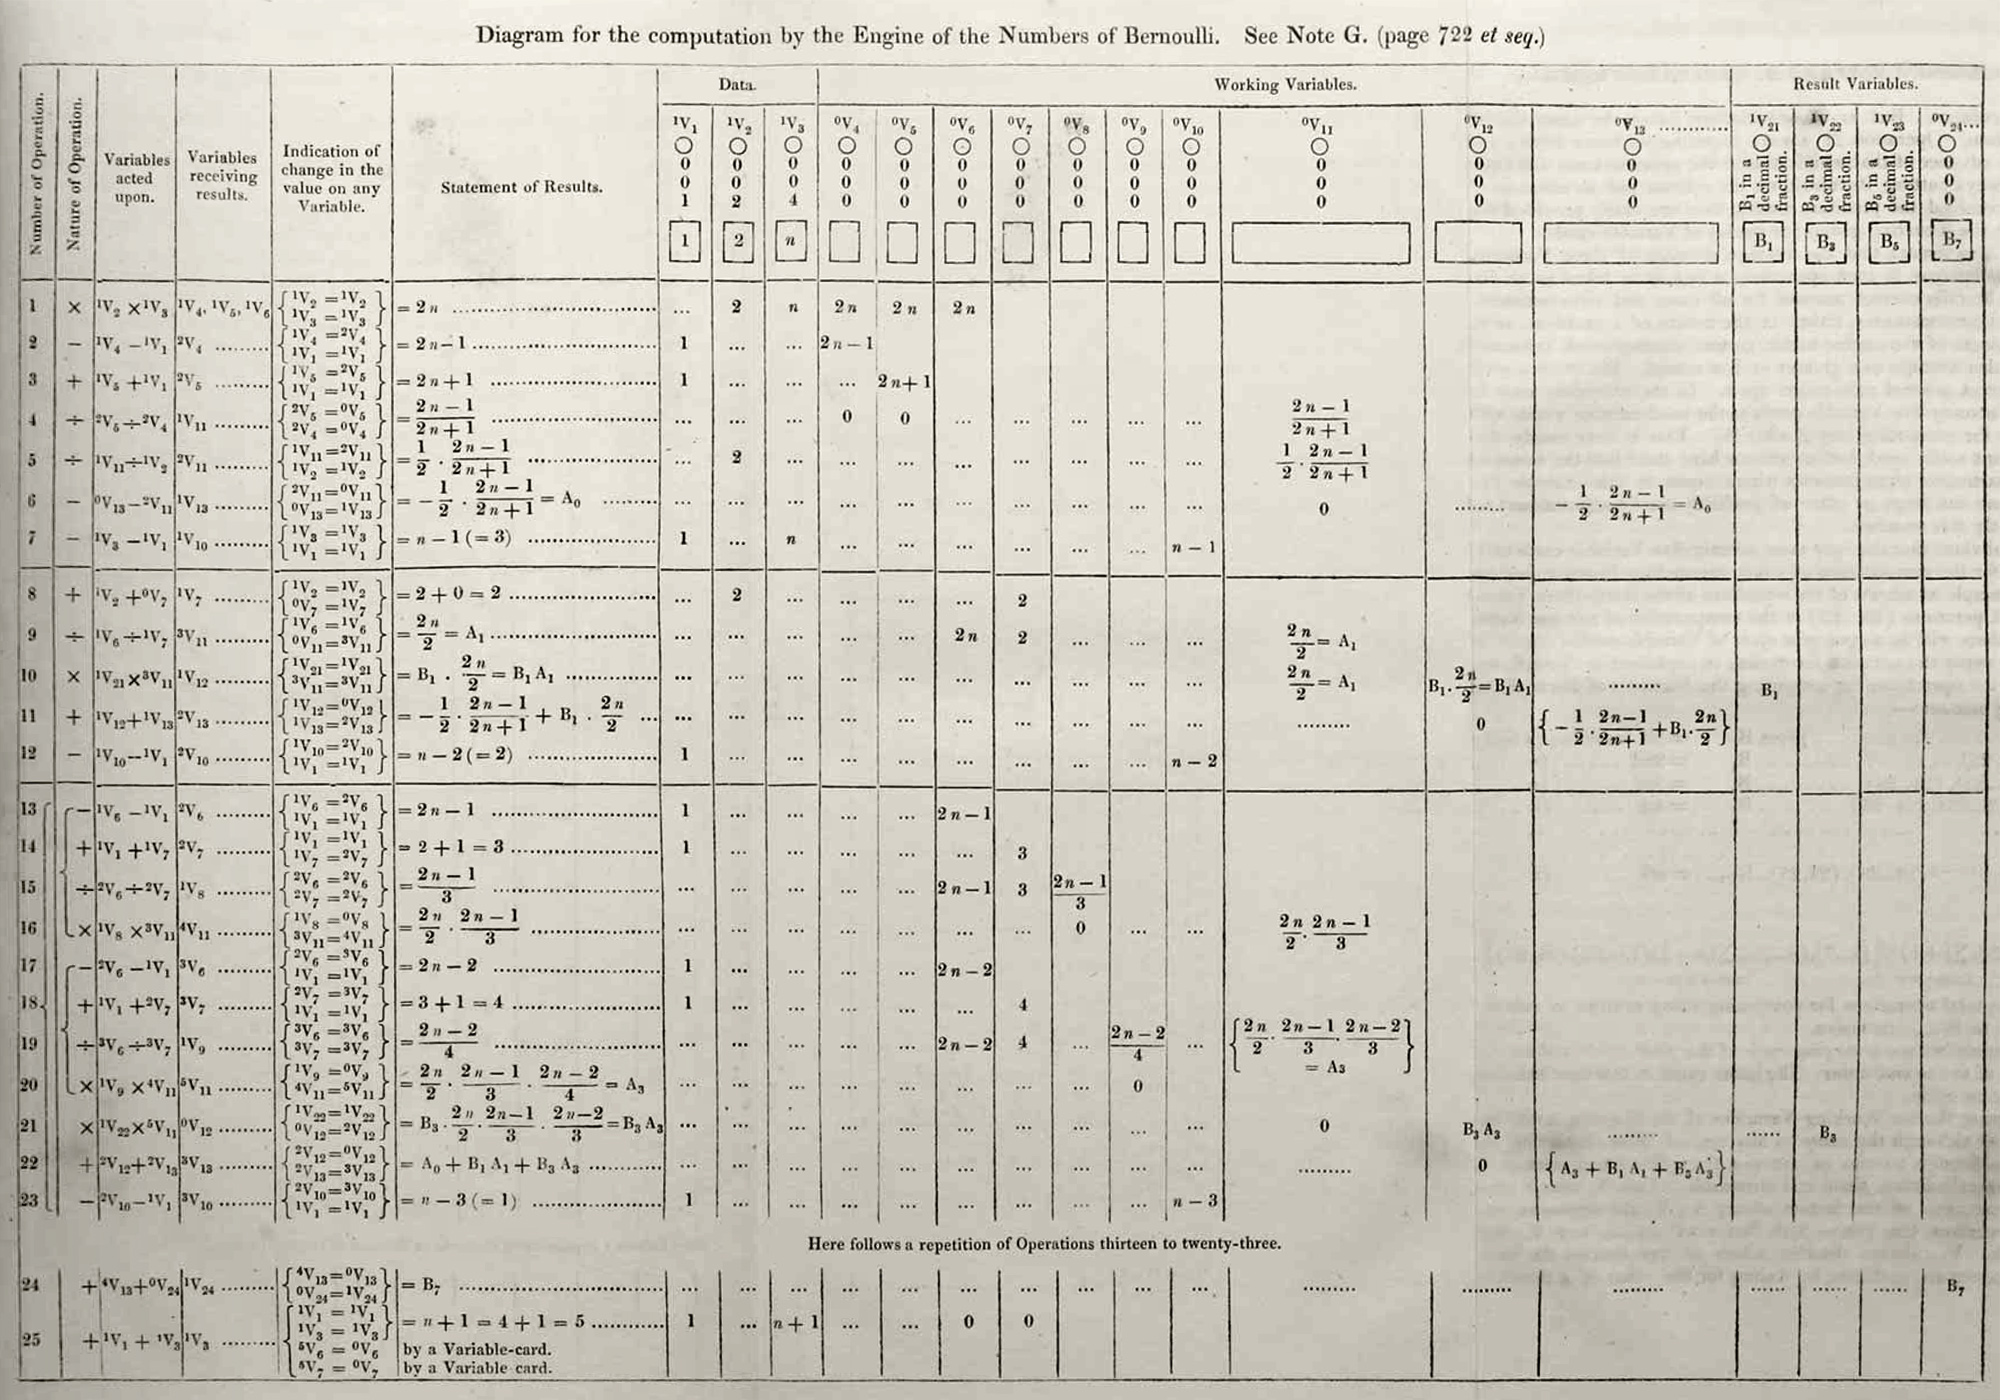
\includegraphics[width=3cm]{first-program}
\addtocounter{framenumber}{-1}
{\usebackgroundtemplate{\begin{minipage}{\paperwidth}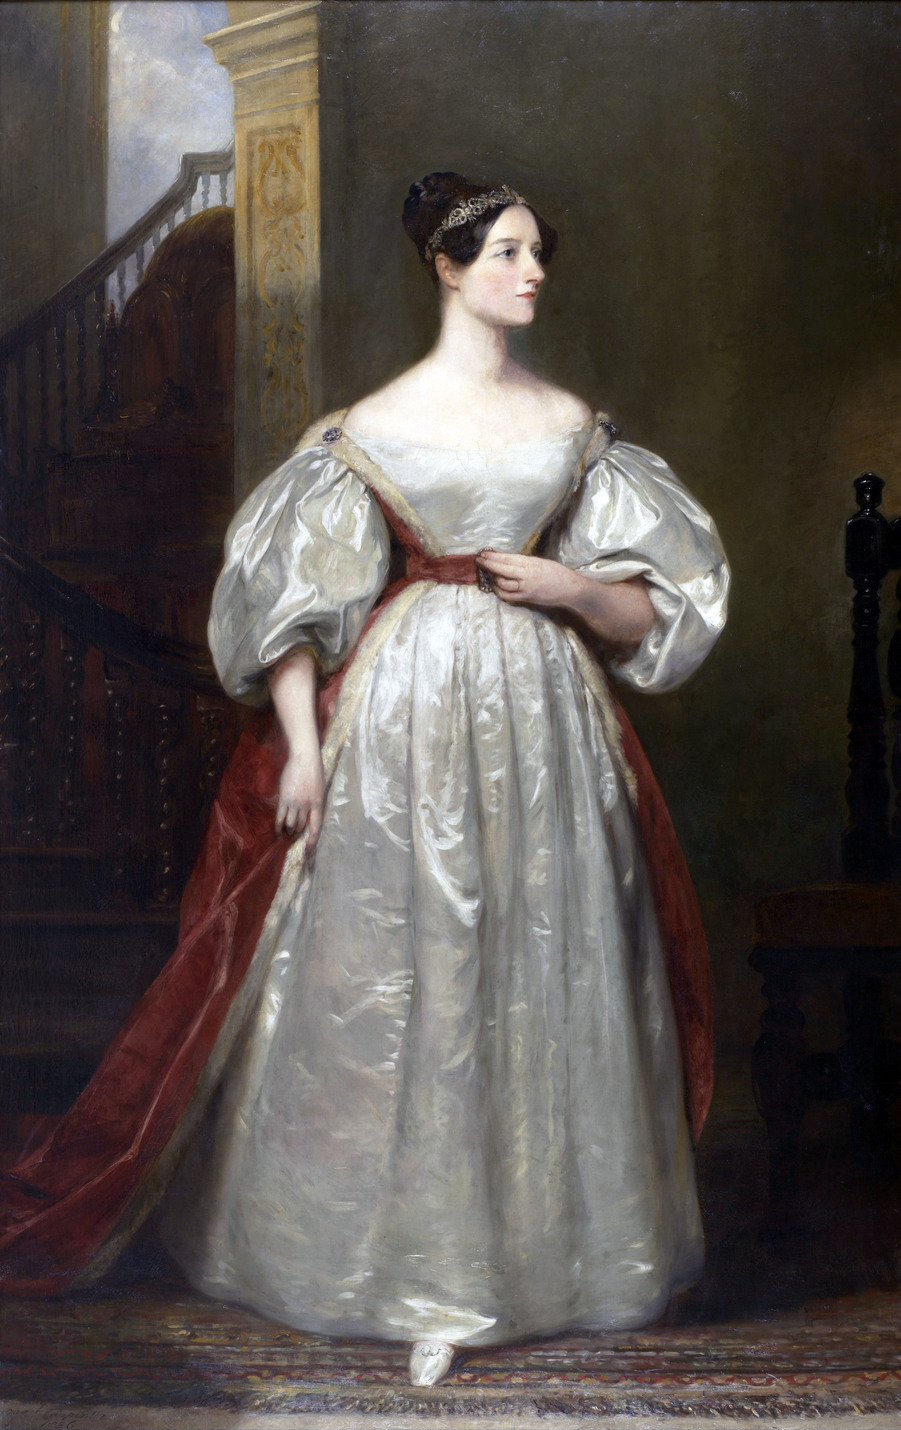
\includegraphics[height=\paperheight,valign=t]{ada-lovelace}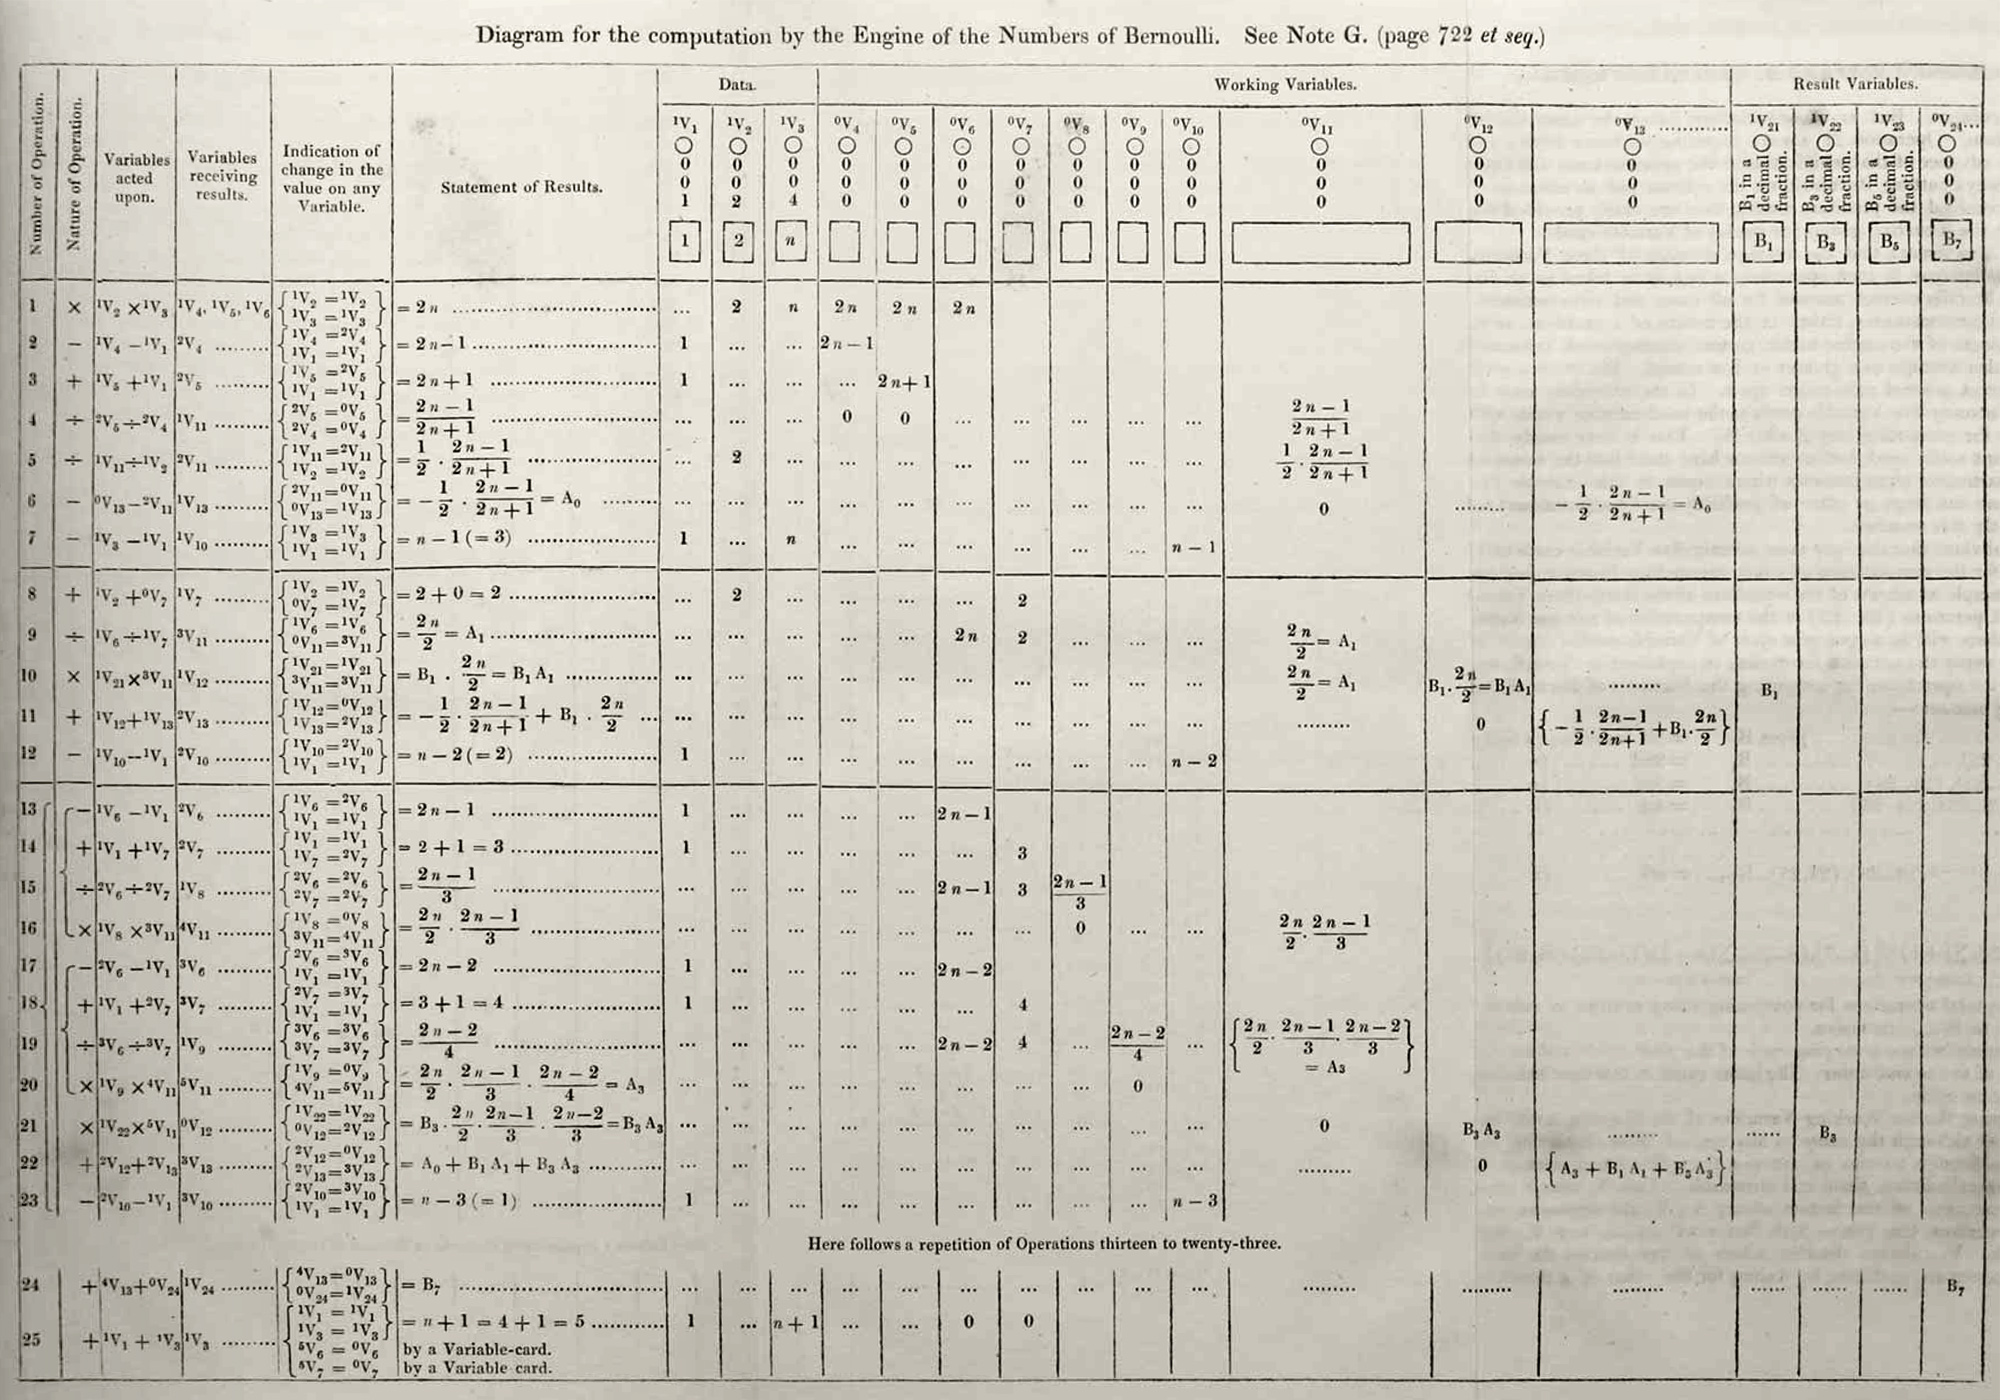
\includegraphics[width=8cm,valign=t]{first-program}\end{minipage}}
\begin{frame}[plain]
  \vspace*{6cm}\hspace*{6cm}\begin{minipage}{4.7cm}
    \huge\hil{Ada Lovelace},

    \Large
    the world's first \\
    computer programmer
    \medskip

    * 1815 \ \ † 1852
  \end{minipage}
\end{frame}}


\section{Realizability theory}

\begin{frame}
  \centering\bigskip
  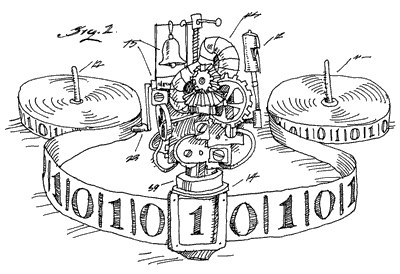
\includegraphics[height=9.5em]{turing-machine}
  \medskip

  \large Lecture I: \\
  \hil{Realizability theory}

  \normalsize

  \emph{for extracting programs from constructive proofs}
\end{frame}

\begin{frame}{Heyting arithmetic}
  The \hil{language of arithmetic} has
  \begin{itemize}
    \item as its single sort: $N$
    \item as function symbols: $0$, $S$, $+$, $\cdot$
    \item as its single relation symbol: $=$
  \end{itemize}

  \hil{Heyting arithmetic} has as axioms (the universal closure of)
  \begin{align*}
    &&& \neg(0 = Sx) \\
    &&& S(x) = S(y) \Rightarrow x = y \\
    x + 0 &= x &&&
    x \cdot 0 &= 0 \\
    x + S(y) &= S(x+y) &&&
    x \cdot S(y) &= (x \cdot y) + x
  \end{align*}
  together with the \hil{induction scheme} (one axiom for each
  formula~$\varphi$)
  \[
    \varphi(0) \wedge \bigl(\forall x\?N\_ \varphi(x) \Rightarrow
    \varphi(S(x))\bigr) \quad\Longrightarrow\quad \forall x\?N\_ \varphi(x)
  \]
  and the rules of \hil{sequence calculus}.
\end{frame}

\begin{frame}{Sequence calculus}
  \begin{center}
    \vspace{-0.5em}
    \phantom{a}\hfill
    \AxiomC{$\phantom{\seq{\vec x}}$}\UnaryInfC{$\varphi \seq{\vec x} \varphi$}\DisplayProof\hfill
    \AxiomC{$\varphi \seq{\vec x} \psi$}\UnaryInfC{$\varphi[\vec s/\vec x]
    \seq{\vec y} \psi[\vec s/\vec x]$}\DisplayProof\hfill
    \AxiomC{$\varphi \seq{\vec x} \psi$}\AxiomC{$\psi \seq{\vec x}
    \chi$}\BinaryInfC{$\varphi \seq{\vec x} \chi$}\DisplayProof
    \phantom{a}\hfill
    \bigskip\medskip

    \phantom{a}\hfill
    \AxiomC{$\phantom{\seq{\vec x}}$}\UnaryInfC{$\varphi \seq{\vec x} \top$}\DisplayProof\hfill
    \AxiomC{$\phantom{\seq{\vec x}}$}\UnaryInfC{$\varphi \wedge \psi \seq{\vec x} \varphi$}\DisplayProof\hfill
    \AxiomC{$\phantom{\seq{\vec x}}$}\UnaryInfC{$\varphi \wedge \psi \seq{\vec x} \psi$}\DisplayProof\hfill
    \AxiomC{$\varphi \seq{\vec x} \psi$}\AxiomC{$\varphi \seq{\vec x} \chi$}\BinaryInfC{$\varphi \seq{\vec x} \psi \wedge \chi$}\DisplayProof
    \phantom{a}\hfill
    \bigskip\medskip

    \phantom{a}\hfill
    \AxiomC{$\phantom{\seq{\vec x}}$}\UnaryInfC{$\bot \seq{\vec x} \varphi$}\DisplayProof\hfill
    \AxiomC{$\phantom{\seq{\vec x}}$}\UnaryInfC{$\varphi \seq{\vec x} \varphi \vee \psi$}\DisplayProof\hfill
    \AxiomC{$\phantom{\seq{\vec x}}$}\UnaryInfC{$\psi \seq{\vec x} \varphi \vee \psi$}\DisplayProof\hfill
    \AxiomC{$\varphi \seq{\vec x} \chi$}\AxiomC{$\psi \seq{\vec x} \chi$}\BinaryInfC{$\varphi \vee \psi \seq{\vec x} \chi$}\DisplayProof
    \phantom{a}\hfill
    \bigskip\medskip

    \phantom{a}\hfill
    \Axiom$\varphi \wedge \psi\ \fCenter\seq{\vec x} \chi$
    \doubleLine
    \UnaryInf$\varphi\ \fCenter\seq{\vec x} \psi \Rightarrow \chi$
    \DisplayProof
    \phantom{a}\hfill
    \bigskip\medskip

    \phantom{a}\hfill
    \Axiom$\varphi\ \fCenter\seq{\vec x, y} \psi$
    \doubleLine
    \UnaryInf$\exists y\?Y\_\! \varphi\ \fCenter\seq{\vec x} \psi$
    \DisplayProof
    {\tiny ($y$ not occurring in~$\psi$)}
    \hfill
    \Axiom$\varphi\ \fCenter\seq{\vec x, y} \psi$
    \doubleLine
    \UnaryInf$\varphi\ \fCenter\seq{\vec x\phantom{, y}} \forall y\?Y\_\! \psi$
    \DisplayProof
    {\tiny ($y$ not occurring in~$\varphi$)}
    \hfill\phantom{a}

    \phantom{a}\hfill
    \AxiomC{$\phantom{\seq{\vec x}}$}
    \UnaryInfC{$\top \seq{x} x = x$}
    \DisplayProof
    \hfill
    \AxiomC{$\phantom{\seq{\vec x}}$}
    \UnaryInfC{$(\vec x = \vec y) \wedge \varphi \seq{\vec z} \varphi[\vec y/\vec x]$}
    \DisplayProof
    \hfill\phantom{a} \\[0.5em]
    (``$\vec x = \vec y\,$'' is short for~``$x_1 = y_1 \wedge \cdots \wedge x_n =
    y_n$''.)
  \end{center}
\end{frame}

\newcommand{\realizes}{\Vdash}

\begin{frame}{Number realizability}
  \vspace*{-1em}
  \begin{changemargin}{-1.5em}{-0.5em}
  \begin{tabbing}
    $e \models (\forall f\?\NN^\NN\_ \varphi(n))$ \= \kill
    $e \realizes s = t$ \> iff $s = t$. \\
    $e \realizes \top$ \> iff true. \\
    $e \realizes \bot$ \> iff false. \\
    $e \realizes (\varphi \wedge \psi)$ \> iff~$\pi_1 \cdot e \downarrow$
    and~$\pi_2 \cdot e \downarrow$ and $\pi_1 \cdot e \realizes \varphi$
    and~$\pi_2 \cdot e \realizes \psi$. \\
    $e \realizes (\varphi \vee \psi)$ \> iff~$\pi_1 \cdot e \downarrow$
    and~$\pi_2 \cdot e \downarrow$ and \\ \> \qquad if~$\pi_1 \cdot e = 0$
    then~$\pi_2 \cdot e \realizes
    \varphi$, and \\ \> \qquad if~$\pi_1 \cdot e \neq 0$ then~$\pi_2 \cdot e \realizes \psi$. \\
    $e \realizes (\varphi \Rightarrow \psi)$ \> iff for every~$r \in \NN$
    such that~$r \realizes \varphi$, $e \cdot r \downarrow$ and~$e \cdot r \realizes \psi$. \\
    $e \realizes (\forall n\?N\_ \varphi(n))$ \> iff for every~$n_0
    \in \NN$, $e \cdot n_0 \downarrow$ and~$e \cdot n_0 \realizes \varphi(n_0)$. \\
    $e \realizes (\exists n\?N\_ \varphi(n))$ \> iff~$\pi_1 \cdot e
    \downarrow$ and~$\pi_2 \cdot e \downarrow$
    and~$\pi_2 \cdot e \realizes \varphi(\pi_1 \cdot e)$. \\
    $e \realizes (\forall f\?N^N\_ \varphi(f))$ \> iff for every~$f_0
    : \NN \to \NN$ and every~$r_0 \in \NN$ such that \\ \> \qquad $f_0$ is computed by the~$r_0$-th
    machine, \\ \> \qquad
    $e \cdot r_0 \downarrow$ and~$e \cdot r_0 \realizes \varphi(f_0)$. \\
    $e \realizes (\exists f\?N^N\_ \varphi(f))$ \> iff~$\pi_1 \cdot e \downarrow$
    and~$\pi_2 \cdot e \downarrow$ and
    the $(\pi_1 \cdot e)$-th machine \\ \> \qquad computes a function~$f_0 : \NN \to \NN$
    and $\pi_2 \cdot e \realizes \varphi(f_0)$.
  \end{tabbing}\end{changemargin}

  \mbox{\textbf{Thm.} If~$\text{HA} \vdash \varphi$, then there is a
  number~$e \in \NN$ such that~\only<1>{$e \realizes
  \varphi$}\only<2>{$\text{HA} \vdash (\underline{e} \realizes \varphi)$}.}
\end{frame}

% \begin{document}

\newcommand{\expl}[2]{
  \justifying
  ``$\realizes \!\text{\normalnumber{#1}}$'' amounts to: #2
}

\newcommand{\qswitch}[3]{\only<1-#1>{
\includegraphics[height=0.7em]{question-mark}}\only<#2->{#3}}
\newcommand{\ccmark}{\good{\cmark}}
\newcommand{\cxmark}{\bad{\xmark}}

{\usebackgroundtemplate{\begin{minipage}{\paperwidth}\vspace*{0.00cm}\hfill\mbox{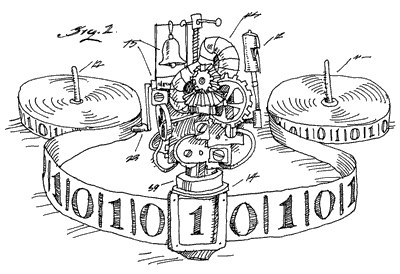
\includegraphics[width=0.2\textwidth]{turing-machine}\;\;}\end{minipage}}
\begin{frame}{Exploring the realizability model}
  \medskip
  \medskip
  \medskip
  \begin{tabular}{@{\!\!\!\!\!\!\!}l@{\,}llp{1.8cm}}
    \toprule
    & Statement & classical? & realizable? \\
    \midrule
    \normalnumber{1} & Every number is prime or not prime. & \ccmark{}
    (trivially) & \ccmark \\
    \normalnumber{2} & After every number there is a prime. & \ccmark & \ccmark \\
    \normalnumber{3} & Every map $\NN \to \NN$ has a zero or not. & \ccmark{} (trivially) & \cxmark \\
    \normalnumber{4} & Every map $\NN \to \NN$ is computable. & \cxmark &
    \qswitch{4}{5}{\ccmark}\only<1-4>{\,} \visible<5->{(trivially)} \\
    \normalnumber{5} & Every map $\RR \to \RR$ is continuous. & \cxmark &
    \qswitch{5}{6}{\ccmark} \\
    \normalnumber{6} & Markov's principle holds. & \ccmark{} (trivially) &
    \qswitch{6}{7}{\ccmark{} (if MP)} \\
    \normalnumber{7} & Countable choice holds. & \ccmark &
    \qswitch{7}{8}{\ccmark{} (always!)} \\
    \normalnumber{8} & Heyting arithmetic is categorical. & \cxmark &
    \qswitch{8}{9}{\ccmark{} (if MP)} \\
    \bottomrule
  \end{tabular}
  \medskip

  \only<1>{\ \\\ \\\ \\\ }
  \only<2>{\expl{1}{There is a machine which determines of any given
  number whether it is prime or not. \\\ }}
  \only<3>{\expl{2}{There is a machine which, given a number~$n$, computes a
  prime larger than~$n$. \\\ \\\ }}
  \only<4>{\expl{3}{There is a machine which, given a machine
  computing a map~$f : \NN \to \NN$, determines whether~$f$ is constantly
  zero or not. \\\ }}
  \only<5>{\expl{4}{There is a machine which, given a machine
  computing a map~$f : \NN \to \NN$, outputs a machine
  computing~$f$. \\\ }}
  \only<6>{\ \\\ \\\ \\\ }
  \only<7>{\expl{6}{There is a machine which, given a machine
  computing a map~$f : \NN \to \NN$ and given the promise that it is \notnot
  the case that~$f$ has a zero, determines a zero of~$f$.}}
  \only<8->{\expl{7}{\justifying There is a machine which, given a machine
  computing for every~$x \in \NN$ some~$y \in A$ together with a realizer
  of~$\varphi(x,y)$, outputs a machine computing a suitable choice
  function~$\NN \to A$.}}
\end{frame}}

\begin{frame}{Metatheory of Heyting arithmetic}
  \begin{enumerate}
    \item \hil{Unprovability results:}
    \medskip

    There are instances of~\badbox{\textsc{lem}} which HA does not prove,
    such as ``every Turing machine terminates or does not terminate''.
    \bigskip

    \item \hil{Disjunction property:}
    \medskip

    If HA proves~$\varphi \vee \psi$, then HA
    proves~$\varphi$ or HA proves~$\psi$.
    \bigskip

    \item \hil{Existence property:}
    \medskip

    If HA proves~$\exists n\?N\_ \varphi(n)$, then there is a number~$n_0 \in
    \NN$ such that HA proves~$\varphi(\underline{n_0})$.
    \bigskip

    \item \hil{Growth rate:}
    \medskip\justifying

    If HA proves~$\forall x\?N\_ \exists y\?N\_ \varphi(x,y)$,
    then there exists a \hil{higher primitive recursive} function $f_0 : \NN
    \to \NN$ such that for all~$x_0 \in \NN$, HA proves
    $\varphi(\underline{x_0}, \underline{f_0(x_0)})$.
  \end{enumerate}
\end{frame}

\begin{frame}{Range of machine models}
  \begin{enumerate}
    \item \hil{Turing machines}

    \visible<2->{``Every function $\NN \to \NN$ is computable'' is realized by
    \textsf{cat}.}
    \medskip

    \item \hil{Untyped lambda calculus}

    \visible<3->{``Every function $\NN \to \NN$ is computable'' is \emph{not}
    realized.}
    \medskip

    \item \hil{Infinite-time Turing machines}

    \visible<4->{``Every function $\NN \to \NN$ has a zero or not'' is realized by
    infinite search.}
    \medskip

    \item \hil{Gödel's System T}

    \visible<5->{Markov's principle is not realized.}
    \medskip

    \item \hil{Machines in the real world} -- philosophical

    \justifying
    \visible<6->{``Every function $\RR \to \RR$ is continuous'' is realized if,
    in the physical world, only finitely many computational
    steps can be carried out in finite time and if it is possible to form
    tamper-free private communication channels.}
  \end{enumerate}
\end{frame}

\end{document}

start:
- infinitude of primes
- Dickson's lemma
- "Every constructive theorem has a computable witness."
- induction = recursion, Markov = unbounded search, ...
- side effects
- applications:
  - integrated developments (for instance SAT checking)
  - metatheory of constructive systems
  - philosophy
  - exploring computability theory

definition:
- HA
- TM
- realizability (as formalization of BKH)
- proof

examples:
- as in filmat paper
  - also with lambda terms!

special kinds of statements:
- negated: uninformative
- double negation
- Π⁰₁

metatheory of HA:
- disjunction property
- existence property
- unprovability of (for instance) halting
- growth rate

variants:
- ITTM
- real world
- completion to Eff

----

- play
- double-negation embedding
- Friedman's trick
- perhaps in Agda

\begin{block}{}
  \justifying
  \textbf{Thm.}
  Every pair of infinite sequences~$\alpha,\beta : \NN \to \NN$ is \emph{good} in that
  there are~$i < j$ such that~$\alpha(i)
  \leq \alpha(j)$ and~$\beta(i) \leq \beta(j)$.
\end{block}
\vspace*{-0.6em}
{\small\emph{Proof.} By~\badbox{\textsc{lem}}+\badbox{\textsc{dc}}, there is a
monotonic subsequence
\[ \alpha(i_0) \leq \alpha(i_1) \leq \alpha(i_2) \leq \cdots \]
with~$i_0 < i_1 < \cdots$. By~\badbox{\textsc{lem}}, there is a minimal
value~$\beta(i_{k_0})$ among all values of~$(\beta(i_k))_k$. Then
$\alpha(i_{k_0}) \leq \alpha(i_{k_0+1})$ and
$\beta(i_{k_0}) \leq \beta(i_{k_0+1})$. \qed
\par}
